\documentclass{llncs}

\usepackage{url}
\usepackage{graphicx}
\usepackage{listings}
\usepackage{verbatim}
\usepackage[lined,linesnumbered,algochapter]{algorithm2e}
\usepackage{tikz}
\usetikzlibrary{arrows,automata}
\usepackage{xspace}
\usepackage{todonotes}          % Package for working draft comments
\usepackage{hyperref}           % Package for hyperlink references in the document

\usepackage[english]{babel}

\setcounter{secnumdepth}{2}
\setcounter{tocdepth}{3}

% define custom macros for specific formats or names
\newcommand{\uml}[1]{\texttt{#1}}
\newcommand{\cd}{\textsf{Class Diagram}}

\begin{document}
\pagestyle{plain}
\pagenumbering{roman}

\title{Refactoring UML models}
\author{Kristof Meixner}
\institute{\email{kristof.meixner@fatlenny.net} \\ Registration No. 9725208}

\maketitle

\begin{abstract} Over the last twenty years refactoring advanced to a commonly known and used technique in modern
software engineering. We present an overview from the beginning of refactoring in code centric software development to its actual application
in model-driven software development. Furthermore, we discuss methods that ensure that refactored models are still formally 
correct after refactoring modifications, such as static and dynamic analysis. We present research on fUML a subset of UML that precisely defines the semantics 
for execution of models and thus enables dynamic testing. At the end we introduce some work, that can be adapted in order to
implement refactorings that are applied on class diagrams and have side effects on corresponding activity diagrams.
\end{abstract}


\tableofcontents
%\thispagestyle{plain}
\newpage

\pagenumbering{arabic}

\section{Introduction}
\label{sec:intro}

Model-based software development or model-driven software development is not only an extensive field of research but
receives also more and more attention from the industry. Nowadays models are not only used as visual explanations of
the underlying concepts but as source for the software development process itself. Thus models need to provide an abstraction of the
represented concepts in high quality. To provide quality assured software artifacts that stay adjustable and reusable during the complete software development
life-cycle, a technique called refactoring is often used to restructure artifacts, which are in our case models. Refactoring should improve
the quality and also the understandability of the models as well as adapt the models to changes arising from the
domain. The most important requirement for refactorings is that they preserve the behavior of the model. In our project
work we focus on an set of refactorings that should be implemented taking the correlations between different model types
as well as static and dynamic analysis into account. In this work we concentrate on the related work in a broader sense
and present them in a chronological manner.

The paper is structured as follows. Section \ref{sec:beginning} copes with the early works on refactoring in the domain
of source code development. Section \ref{sec:fromto} presents how commonly known refactorings from source code where
adapted in theoretical works to models and how they can be tested for correctness with static methods. Section 
\ref{sec:todynamics} discusses actual research on how models can also be tested dynamically by executing and debugging 
the models. Finally Section \ref{sec:conclusion} summarizes the presented research.

\section{Beginning in refactoring}
\label{sec:beginning}

In this section we will present an overview on the beginnings in structured refactoring of source code. In his thesis
Opdyke \cite{mast:REFOOF} defines refactoring as a set of operations that restructure an artifact but at the same time
preserve the behavior to increase software quality. This technique became known as refactoring.

The motivation of his work is on the one hand that software should be reused because of the high costs of development
and on the other hand that software needs to be restructured over its life-cycle to maintain this reusability. The issue
he addressed in his work is the problem of changing parts of source code of an object-oriented system, grounded in a
possibly large code base while also maintaining all the references and dependencies manually. He described this a time
consuming process which is difficult and leaves room for further errors. As a solution he proposes an automated support
for refactoring which means ``plans'' to reorganize the source code on an intermediate level without changing the behavior
of the program.

A section in the thesis covers behavior preserving approaches. In this section he first mentions the usage of
\textit{preconditions} to ensure that a refactoring does not corrupt the syntax and more important does not change the
execution behavior of the program. He quickly refuses the approach to use the static compiler to test these issues as
the compiler is not capable to catch errors that change the behavior. In this section also some rules are presented that
can be tested beforehand to check whether a refactoring is possible on the source code. An important rule to mention copes with
semantic preservation of code and is described as ``Semantically Equivalent References and Operation'' \cite{mast:REFOOF}. He there defines
semantic equivalence such that a call of an interface with the same set of input values should result in the same set of
output values despite any change of the interals of the program. This means that from outside of a part of the specific system
the refactoring is not visible. The range of this part to be considered, however, differs from the impact of the refactoring on
the system. In the rest of his work he shows some examples of refactorings depending on their level of implication on
the source code for \textit{Smalltalk} program concepts and how they could be applied.

Roberts \cite{rob99}, writing his thesis at the same University, builds large parts of his contribution on the work of
Opdyke. He criticizes that the refactorings described by Opdyke are too small and cannot be performed as a single
operation but often need to be done in a sequence of steps to refactor the code to a better ``design in mind''.  He also mentions
that the costly analysis for legal code after a refactoring should be eliminated and introduces postconditions along
with Opdykes preconditions to guarantee behavior preservation. Besides his contribution of a definition of refactoring
that also uses \textit{postconditions}, Roberts presents a dependency definition of refactorings that is based on the
commutativity of single changes applied in sequence. Furthermore he presents an idea, which in our work seems rather interesting,
to analyze very complex refactorings not in a static manner but dynamically during execution. This in
particular fits to later work in this field that builds on executing models and revealing changes due to refactoring before
and after the modification. Roberts also redefines the refactorings developed by Opdyke and presents his catalog that
can be used as a source for modern refactoring.

Another extensive catalog of refactorings based on source code in \textit{Java} was developed and
described by Fowler in \cite{fow99}. His list of refactorings\footnote{The catalog can be found online at
http://refactoring.com/catalog/} is continuously updated and extended for different programming language and shows also
good examples of how to refactor a program in design pattern thinking.

\section{From source code to model refactoring}
\label{sec:fromto}

In the last section we gave a brief introduction to the early research in refactoring of source code. In this section we will discuss
what model refactoring is and how it can be build upon the approaches developed for source code refactoring. 

As already mentioned in Section
\ref{sec:intro}, modern software development more and more uses the concepts of model-based and model-driven approaches
which means that formal models are one of the most important artifacts in development. This also implies that changes in
the domain of the software have to be propagated to the formal models. With faster development cycles common in agile
software development like eXtreme programming \cite{DBLP:journals/computer/Beck99} or Scrum
\cite{DBLP:journals/software/RisingJ00} those changes have to be done even more efficient and reliable. It is obvious
that in this case model development benefits from the available techniques of refactoring introduced in the late nineties for
source code. However, models need to be treated differently than source code.

\begin{figure}[h!t]
 \centering
 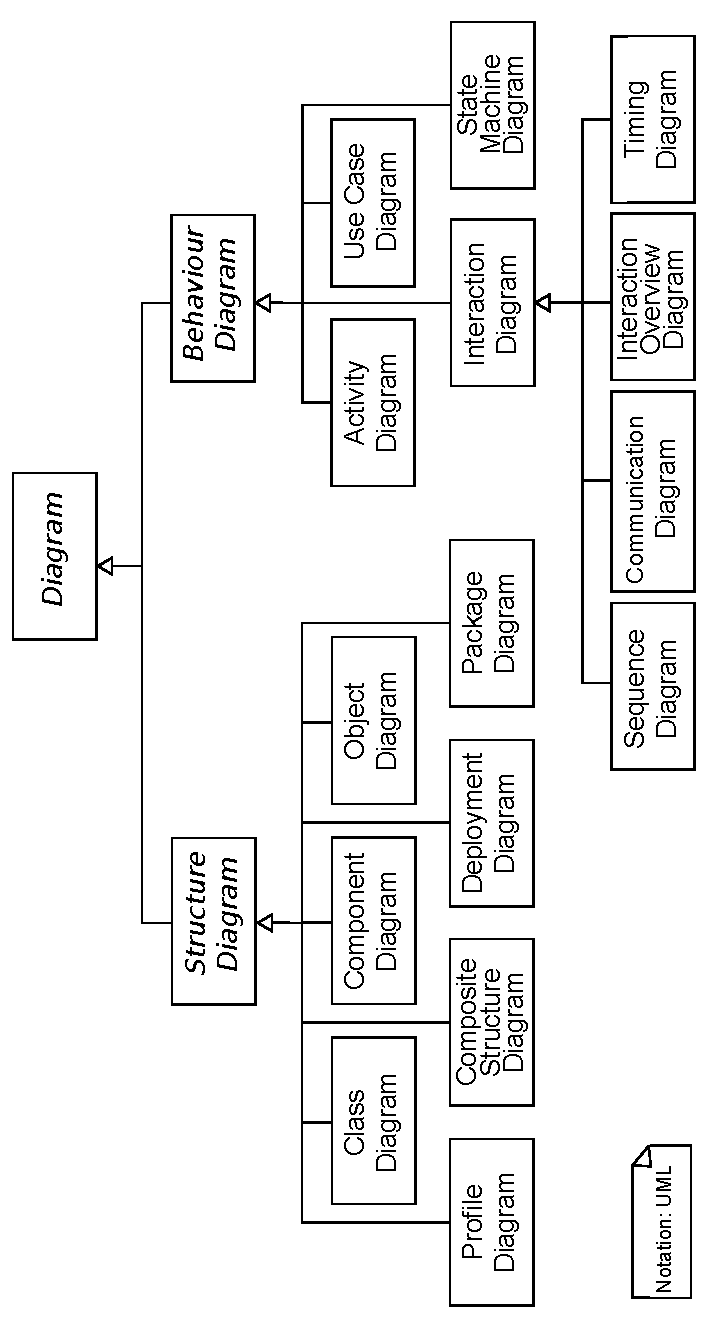
\includegraphics[scale=0.54,angle=270]{images/uml}
 \caption{UML diagram type hierarchy (Wikipedia)}
 \label{fig:uml}
\end{figure}

Today the de-facto standard for modeling software systems is the \textit{Unified Modeling Language} (UML) \cite{man:UML} standardized by the
\textit{Object Management Group}\footnote{http://www.omg.org/} (OMG) in 1997. It is a general purpose language used
for model creation and development. UML consists of an abstract syntax which builds the foundations for creating 
models which are represented in the concrete syntax of the language. UML defines several different diagram types
that can be used for designing parts of a software system. The most commonly used diagram type is the class diagram
which is often used to depict models and components of software architecture. Generally the diagrams can be categorized
into structural and behavioral diagrams. A further partitioning of the diagrams is shown in Figure \ref{fig:uml}. The
different diagrams share a common meta-model in the background and are usually serialized in \textit{XML Metadata
Interchange} (XMI) format \cite{man:XMI} an \textit{XML} exchange format which is also
standardized by the OMG.

The OMG furthermore defined the \textit{Object Constraint Language} (OCL) \cite{man:OCL} which is a
formal language to annotate UML models with expressions \cite{man:OCL}. The expressions specify mainly
invariants but also preconditions and postconditions that have to hold for the modeled system.

One of the first works in the domain of model refactoring was done by Suny{\'e}~\textit{et al.} 
\cite{DBLP:conf/uml/SunyePTJ01}. They state that refactoring of models is difficult because the impact of changes to the
model is hard to measure. This holds especially for UML as the different model diagram types need to be taken into
account, where modeling elements often spread over views. Suny{\'e}~\textit{et al.} brings up an example of a class diagram and a
state chart diagram and describes how some refactorings can be applied on these models which are verified by pre- and
postconditions formulated in OCL to ensure the preservation of the behavior of the models. The work gives a good idea about how model
refactorings can be achieved and statically tested. However, also the authors state that ``the search for some UML
specific refactorings has been somehow frustrating, specially when we wanted transformations to have an impact on
different UML views'' \cite{DBLP:conf/uml/SunyePTJ01}. We also somehow experienced that most of the reviewed research
concentrated only on refactoring UML class diagrams in their work, reflecting their impact on other parts of the model 
such as activity diagrams.

Gorp~\textit{et al.} \cite{gorp03} in addition to the work before contributed a proposal for the extension of UML in
2003 and the use of code smells in combination with OCL pre- and postconditions to bundle so called
\textit{refactoring contracts}. Code smells are symptoms for design flaws and might indicate problems that are hidden
deeper in the source code. Gorp recommended to use a threefold process for refactoring. First use preconditions to
verify that a refactoring is possible, second use a code smell detector to find smells that indicate that the model 
benefits from a refactoring and last but not least use the postconditions for a final check. In their research they
adapted the method for two refactorings namely \textit{pullup method} and \textit{extract method}.

Markovic and Baar \cite{DBLP:journals/sosym/MarkovicB08} examined how refactorings of UML class diagrams affect their
defined OCL constraints. They presented a catalog of refactorings that leans on the catalog of Fowler and classify
them by their impact on the abstract syntax representation of the models. In their work they state that simple refactorings
might be easy to track and impacts may be traced and addressed on the fly. However, if the abstract syntax representation
changes, the refactorings can result in complex changes of the model and the corresponding class diagram as well as OCL
constraints. They therefore formalize their refactoring rules in a graphical notation included in the
\textit{QVT} \cite{man:QVT} standard by the OMG. The grapical representation is divided
in a left hand side \textit{LHS} and a right hand side \textit{RHS}. The LHS shows the original state of the model
in abstract syntax and the preconditions, which have to be met such that the refactoring can be applied. The RHS shows
the state of the model after the refactoring. They also present an implementation of the refactorings in
\textit{Eclipse}\footnote{http://www.eclipse.org/}.

The last work we discuss in this section is the one of Arendt and Taentzer \cite{DBLP:conf/models/ArendtTW13}.
Arendt and Taentzer relied on the work of Mohagheghi~\textit{et al.} \cite{DBLP:journals/infsof/MohagheghiDN09} that condensed
six classes of quality goals in model development out of several studies. These are \textit{Correctness},
\textit{Completeness}, \textit{Consistency}, \textit{Comprehensibility}, \textit{Confinement} and
\textit{Changeability}. With these goals in mind they formulated a set of questions that can be checked for specific
models and show possible smells in the underlying concepts. Furthermore they implemented a complete framework based
on the \textit{Eclipse Modeling Framework} \cite{Steinberg:2009:EEM:1197540} called \textit{EMF
Refactor}\footnote{http://www.eclipse.org/emf-refactor/}. This plugin to Eclipse allows to calculate defined
metrics and smells for a given model. The user can then choose from various refactorings how to improve the
model and make it more understandable. The framework can be easily extended and supports a wide range of technologies
that can be used to implement further refactorings. Besides the already mentioned buildin module OCL,
additional modules can be created in \textit{Java}, \textit{Henshin}\footnote{https://www.eclipse.org/henshin/} a
transformation engine for \textit{EMF} and \textit{ComRel} ``a model-based language for the combination of EMF model
refactorings'' \cite{DBLP:journals/infsof/MohagheghiDN09}.

\section{From static to dynamic testing}
\label{sec:todynamics}

In the section above we presented some work that covers refactoring of models and uses different methods of static
analysis to ensure that the behavior of the models are preserved and to identify models that were not well designed. In
this section we will discuss research that adapts the approach presented by \cite{rob99} and uses the execution of
systems to dynamically verify that the behavior of a model was preserved by a refactoring.

UML does not provide the semantics to make a model as executable as program code is. This issue was addressed in
the definition of a subset of UML that precisely defines the execution semantics of a subset of UML. This
subset is defined in the standard ``Semantics of a Foundational Subset for Executable UML Models'' (fUML) 
\cite{man:FUML}. It contains concepts of the packages \textit{Classes}, \textit{CommonBehaviors}, \textit{Activities} and \textit{Actions}, which, 
if you recall Figure \ref{fig:uml},  basically means that it is possible to create 
\textit{class diagrams} and \textit{activity diagrams} with fUML. The class diagram can be used to model the domain with its concepts, the activity diagram can be used
to describe the behavior of the concepts in the class diagram.

\begin{figure}[h!t]
 \centering
 \makebox[\textwidth]{
 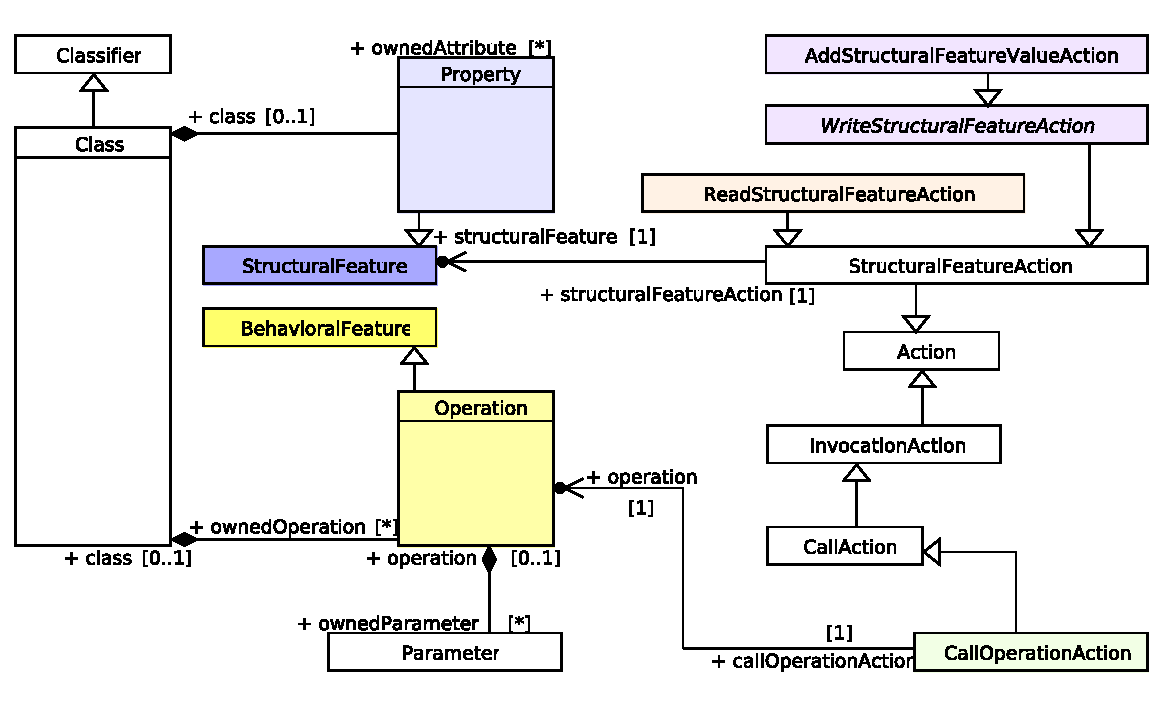
\includegraphics[scale=0.62]{images/Model_Model_Classifiers}
 }
 \caption{Abstract syntax for the used class and behavioral concepts in fUML}
 \label{fig:fuml1}
\end{figure}

In our work we concentrate on this subset to investigate the changes that are implied in the corresponding
diagram if the other diagram changes. In particular we examined which co-refactorings of activity diagrams 
have to be applied when a class diagram is refactored, in order to preserve the executability of the model 
and its behavior. In order for the reader to get more insights on the topic, we provide an example refactoring, namely \textit{encapsulate property}. 
The refactoring is commonly known from source code refactoring and has the following steps:

\begin{itemize}
 \item Create setters and getters for the property.
 \item Change all occurrences of the property to the created setters and getters.
 \item Change the visibility of the property to private.
\end{itemize}

In Figure \ref{fig:fuml1} parts of the abstract syntax for defining classes in class diagrams and activities in activity diagram are
displayed. For the class diagram, there are nearly no modifications necessary except to create the new methods and set the
property's visibility to private. The implied co-refactorings, to access the encapsuled property in an activity diagram, are not that 
obvious. Figure \ref{fig:calculatePremiumRef} shows a very
simple activity diagram. Each of the actions \texttt{read\-Number\-Of\-Vehicles}, \texttt{read\-Customer} and
\texttt{readAge}, displayed in pink in the figures, are actions of type \texttt{Read\-Structural\-Feature\-Action} which read \texttt{Structural\-Features}. 
Each of these actions has to be changed to actions of type \texttt{Call\-Operation\-Action} as they
accessed the property which is not accessible anymore directly, but only via the newly introduced setter and getter operations,
shown in green in Figure \ref{fig:fuml1}. For the new operations also new activities have to be created and their internal 
representations need to be defined. Furthermore, all \texttt{InputPin}s and \texttt{OutputPin}s within the affected 
activities have to be reassigned from the \texttt{Structural\-Feature\-Action}s to the \texttt{Call\-Operation\-Action}.
It can be seen that even this refactoring which is rather simple to apply in source code can get very complex in a model.

\begin{figure}[h!t]
 \centering
 \makebox[\textwidth]{
 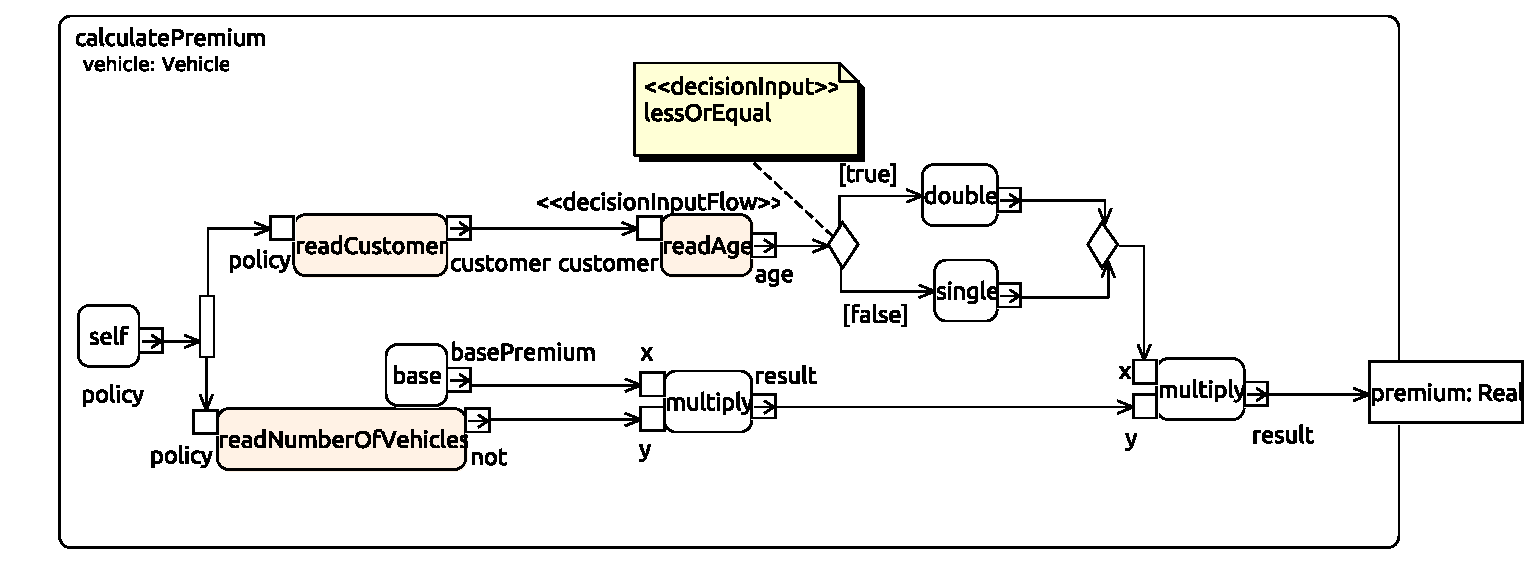
\includegraphics[scale=0.55]{images/insurance_ref/Activity_calculatePremium_calculatePremium}
 }
 \caption{Activity diagram of an example operation \texttt{calculatePremium}}
 \label{fig:calculatePremiumRef}
\end{figure}

Mayerhofer \cite{DBLP:conf/icse/Mayerhofer12} proposes to use common techniques from software development to
dynamically verify the behavior of UML models namely testing and debugging. However some problems come up when
taking a deeper look because ``UML models constitute a multiple view specification of a system reference''. In a further
scientific work by Mayerhofer~\textit{et al.} \cite{DBLP:conf/models/MayerhoferLK12} a runtime model is presented that is capable
to execute and trace activities. They also implemented\footnote{http://www.modelexecution.org/} a virtual machine that
is capable of running fUML models and can even convert UML model compatible to fUML for
execution purposes.

\section{Conclusion}
\label{sec:conclusion}

We presented a brief overview on the scientific work in the domain of refactoring over the last twenty years. It ranges
from source code refactoring with pre- and postconditions and the domain of model-driven development
where refactoring is equally needed but harder to implement because of the different views on the underlying models and
their correlations. Model development tries to take common techniques from source code development and adapt them for
its needs. While from the beginning static analysis was taken into account verifying the correctness of refactorings in the later research and especially with the
standardization of fUML also dynamic analysis like testing and debugging during execution can be exploited.

\newpage
\bibliographystyle{acm}
\bibliography{references}

\end{document}
